%--------------------------------------------------------------
% tesi.tex 
%--------------------------------------------------------------
% Corso di Laurea in Informatica 
% http://if.dsi.unifi.it/
% @Facolt\`a di Scienze Matematiche, Fisiche e Naturali
% @Universit\`a degli Studi di Firenze
%--------------------------------------------------------------
% - template for the main file of Informatica@Unifi Thesis 
% - based on Classic Thesis Style Copyright (C) 2008 
%   Andr\'e Miede http://www.miede.de   
%--------------------------------------------------------------

\documentclass[twoside,openright,titlepage,fleqn,
,	headinclude,12pt,a4paper,BCOR5mm,footinclude,table]{scrbook}
%--------------------------------------------------------------
\newcommand{\myItalianTitle}{Analisi di un sottosistema di posizionamento ferrotramviario\xspace}
\newcommand{\myEnglishTitle}{Analysis of a tramway positioning subsystem\xspace}
% use the right myDegree option
\newcommand{\myDegree}{Corso di Laurea Magistrale in Informatica\xspace}
\newcommand{\myCurriculum}{Resilient and Secure Cyber-Physical System\xspace}
%\newcommand{\myDegree}{
	%Corso di Laurea Specialistica in Scienze e Tecnologie 
	%dell'Informazione\xspace}
\newcommand{\myName}{Alex Foglia\xspace}
\newcommand{\myProf}{Andrea Bondavalli\xspace}
\newcommand{\myOtherProf}{Nome Cognome\xspace}
\newcommand{\mySupervisor}{Nome Cognome\xspace}
\newcommand{\myFaculty}{
	Scuola di Scienze Matematiche, Fisiche e Naturali\xspace}
\newcommand{\myUni}{\protect{
	Universit\`a degli Studi di Firenze}\xspace}
\newcommand{\myLocation}{Firenze\xspace}
\newcommand{\myTime}{Anno Accademico 2018-2019\xspace}
\newcommand{\myVersion}{Version 0.1\xspace}
%--------------------------------------------------------------

\usepackage[italian]{babel}
\usepackage[latin1]{inputenc}
\usepackage[T1]{fontenc} 
\usepackage[square,numbers]{natbib} 
\usepackage[fleqn]{amsmath}  
\usepackage{ellipsis}
\usepackage{listings}
\usepackage{subfig}
\usepackage{caption}
\usepackage{appendix}
\usepackage{siunitx}
\usepackage{url}
\usepackage{placeins}
%--------------------------------------------------------------
\usepackage{dia-classicthesis-ldpkg}
%--------------------------------------------------------------


%
% Options for classicthesis.sty:
% tocaligned eulerchapternumbers drafting linedheaders 
% listsseparated subfig nochapters beramono eulermath parts 
% minionpro pdfspacing
\usepackage[eulerchapternumbers,linedheaders,subfig,beramono,eulermath,
parts]{classicthesis}
%--------------------------------------------------------------
\newlength{\abcd} % for ab..z string length calculation
% how all the floats will be aligned
\newcommand{\myfloatalign}{\centering} 
\setlength{\extrarowheight}{3pt} % increase table row height
\captionsetup{format=hang,font=small}
%--------------------------------------------------------------
% Layout setting
%--------------------------------------------------------------
\usepackage{geometry}
\geometry{
	a4paper,
	ignoremp,
	bindingoffset = 1cm, 
	textwidth     = 13.5cm,
	textheight    = 21.5cm,
	lmargin       = 3.5cm, % left margin
	tmargin       = 4cm    % top margin 
}



%%
%% Julia definition (c) 2014 Jubobs
%%
\lstdefinelanguage{Julia}%
  {morekeywords={abstract,break,case,catch,const,continue,do,else,elseif,%
      end,export,false,for,function,immutable,import,importall,if,in,%
      macro,module,otherwise,quote,return,switch,true,try,type,typealias,%
      using,while,endfor},%
   sensitive=true,%
   alsoother={},%
   morecomment=[l]\#,%
   morecomment=[n]{\#=}{=\#},%
   morestring=[s]{"}{"},%
   morestring=[m]{'}{'},%
}[keywords,comments,strings]%

\lstset{%
    language         = Julia,
    basicstyle       = \ttfamily,
    keywordstyle     = \bfseries\color{blue},
    stringstyle      = \color{magenta},
    commentstyle     = \color{ForestGreen},
    showstringspaces = false,
}
%%%

\usepackage{tikz}
\usetikzlibrary{arrows}
\usetikzlibrary{positioning}
\tikzset{main node/.style={circle,fill=blue!20,draw,minimum size=1cm,inner sep=0pt},
            }



%--------------------------------------------------------------
\begin{document}
\frenchspacing
\raggedbottom
\pagenumbering{roman}
\pagestyle{plain}
%--------------------------------------------------------------
% Frontmatter
%--------------------------------------------------------------


%--------------------------------------------------------------
% titlepage.tex (use thesis.tex as main file)
%--------------------------------------------------------------
\begin{titlepage}
	\begin{center}
   	\large
      \hfill
      \vfill
      \begingroup
         \includegraphics[scale=0.15]{logo/LOGO}\\
%			\spacedallcaps{\myUni} \\ 
			\myFaculty \\
			\myDegree \\ 
			\myCurriculum \\
			\vspace{0.5cm}
         \vspace{0.5cm}    
           
      \endgroup 
      \vfill 
      \begingroup
      	\color{Maroon}\spacedallcaps{\myItalianTitle} \\ $\ $\\
      	\spacedallcaps{\myEnglishTitle} \\ 	
	\bigskip
      \endgroup
      \spacedlowsmallcaps{\myName} \\ $\ $\\
      \myRel \spacedlowsmallcaps{\myProf}
      \vfill 
      \vfill
    
      \vfill
      \vfill
      \myTime
      \vfill                      
	\end{center}        
\end{titlepage}   
%--------------------------------------------------------------
% back titlepage
%--------------------------------------------------------------
   \newpage
	\thispagestyle{empty}
	\hfill
	\vfill
	\noindent\myName: 
	\textit{\myItalianTitle,} 
	\myDegree, \textcopyright\ \myTime
%--------------------------------------------------------------
% back titlepage end
%--------------------------------------------------------------

\pagestyle{scrheadings}
%--------------------------------------------------------------
% Mainmatter
%--------------------------------------------------------------
\pagenumbering{arabic}
% use \cleardoublepage here to avoid problems with pdfbookmark
%\include{intro} % use \myChapter command instead of \chapter
%\cleardoublepage\myPart{Part I}
%\include{chapter01}
%\cleardoublepage\myPart{Part II}
%\include{chapter02}
%\include{chapter03}
\paragraph{Abstract}

\tableofcontents
\listoftables
\listoffigures
\chapter{Stato dell'Arte}
\section{Introduzione}
Negli ultimi anni, i sistemi informatici hanno assunto un ruolo sempre pi\`u centrale nelle attivit\`a umane.\\*
Inizialmente, il computer era considerato un semplice strumento di supporto alla matematica applicata, capace di svolgere calcoli particolarmente onerosi in un tempo relativamente breve. Con lo sviluppo delle tecnologie, i sistemi informatici sono ad oggi impiegati in un vasto insieme di domini applicativi, dall'elettromedicale al trasporto aereo, fino all'\emph{Internet of Things}.\\*
Quanto pi\`u si diffonde l'utilizzo dei sistemi informatici, tanto pi\`u peso assume un eventuale fallimento dei medesimi.\\*
La letteratura scientifica dimostra che la valutazione della \emph{dependability} di un sistema informatico \`e un problema chiave.\\*
Per \emph{dependability} si intende la capacit\`a che ha un sistema di fornire un servizio in modo corretto. \cite{depdef}\\*
Un \emph{fallimento} \`e una transizione compiuta da un sistema dall'erogazione di un servizio corretto verso l'erogazione di un servizio scorretto. La transizione contraria \`e detta \emph{restauro}.\\*
\begin{figure}[h]
	\centering
	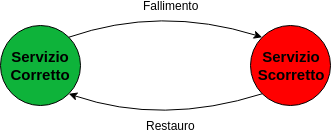
\includegraphics[width=0.7\linewidth]{img/FallimentoRestauro}
	\caption{Fallimento e restauro}
	\label{fig:fallimentorestauro}
\end{figure}\newpage
Effettuare misure sperimentali su un sistema informatico, o su un suo prototipo, \`e una valida opzione per valutarne la \emph{dependability}.\\*
\subsection{Dependability}
La \emph{dependability} di un sistema \`e:
\begin{itemize}
	\item Misurata rispetto a un certo insieme di propriet\`a note come \emph{measures};
	\item Raggiunta attraverso l'utilizzo di specifiche tecniche, i \emph{means};
	\item Minacciata dai \emph{threats}, ossia da tutto ci\`o che porta il sistema ad erogare un servizio improprio.\\*
	Un sistema pu\`o fallire nel caso in cui questo non sia conforme alle specifiche, oppure perch\`e le specifiche non descrivono adeguatamente le sue funzioni.\\*
\end{itemize}
La \emph{dependability} di un sistema viene misurata rispetto alle seguenti propriet\`a:
\begin{itemize}
	\item \emph{Availability}: L'alternanza tra la fornitura di un servizio corretto e uno scorretto.
	$$
	A(t) = \begin{cases} 1 & \mbox{se il servizio fornito \`e corretto al tempo t} \\ 0 & \mbox{altrimenti} \end{cases}
	$$
	$\mathbb E[A(t)]:$ probabilit\`a che il servizio fornito sia corretto al tempo $t$
	\item \emph{Reliability}: Capacit\`a di fornire un servizio continuamente corretto in un certo intervallo di tempo.
	$$
	R(t):\mbox{probabilit\`a di fornire un servizio corretto nell'intervallo }[0,t]
	$$
	\item \emph{Safety}: Il tempo medio a un fallimento catastrofico.\\*\\*
	$S(t):$ probabilit\`a che non si verifichi alcun fallimento catastrofico nell'intervallo $[0,t]$\\*\\*
	\item \emph{Time to Failure}: Il tempo che intercorre fra l'ultimo restauro e il successivo fallimento.\\*
	Spesso \`e opportuno considerare il valore atteso di questa grandezza, il \emph{Mean Time to Failure} (MTTF)
	\item \emph{Maintainability}: Il tempo necessario a restaurare il sistema, dopo l'ultimo fallimento. Il valore atteso di questa misura prende il nome di \emph{Mean Time to Repair} (MTTR)
	\item \emph{Coverage}: Probabilit\`a che il sistema sia in grado di tollerare un guasto.
\end{itemize}
La \emph{safety} \`e un' estensione del concetto di \emph{reliability}.\\*
Si definisce uno stato sicuro in cui il sistema:
\begin{itemize}
	\item Fornisce il servizio corretto, oppure
	\item Non fornisce il servizio corretto, ma il fallimento non ha conseguenze catastrofiche sull'ambiente o sulle persone
\end{itemize}
Qualunque fallimento che induca il sistema a fornire un servizio scorretto con conseguenze catastrofiche, viene modellato come una transizione verso uno stato non sicuro. Quando esiste questa possibilit\`a, il sistema viene definito \emph{safety-critical}.\cite{safetycritical}\\*
\begin{figure}[h]
	\centering
	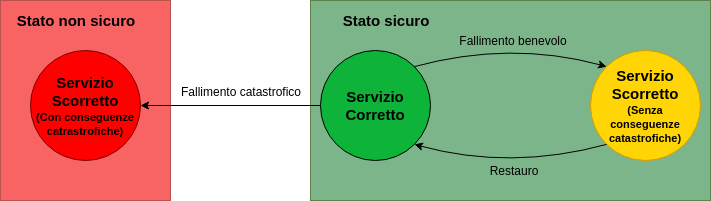
\includegraphics[width=0.7\linewidth]{img/safety}
	\caption{La \emph{safety} estende il concetto di \emph{reliability}}
	\label{fig:safety}
\end{figure}\\*
Esistono numerosi contesti in cui i sistemi impiegati vengono definiti \emph{safety-critical}, uno di questi \`e il trasporto ferroviario.\\*
I \emph{threats} che minano la \emph{dependability} di un sistema sono i guasti, gli errori e i fallimenti.\\*
Un guasto \`e un qualunque evento interno al sistema in grado di causare un errore. Quando l'errore raggiunge l'interfaccia di servizio, ovvero altera il servizio fornito dal sistema, si parla di fallimento. In letteratura, si fa riferimento a questo rapporto di causalit\`a come \emph{fault error failure chain}, catena guasto errore fallimento.\\*
\begin{figure}[h]
	\centering
	
\includegraphics[width=0.7\linewidth]{img/gefpng}
	\caption{Catena guasto errore fallimento}
	\label{fig:gefpng}
\end{figure}\newpage
La \emph{dependability} di un sistema informatico \`e raggiunta attraverso l'uso di quattro tecniche:
\begin{itemize}
	\item \emph{Fault Prevention}: Previene l'insorgenza di guasti durante il ciclo di vita del sistema;
	\item \emph{Fault Tolerance}: Rende il sistema in grado di fornire un servizio corretto anche in presenza di guasti;
	\item \emph{Fault Removal}: Riduce il numero di guasti nel sistema;
	\item \emph{Fault Forecasting}: Stima il numero di guasti presenti nel sistema, attualmente o in futuro;
\end{itemize}
La \emph{dependability} \`e la propriet\`a che viene misurata durante il processo di \emph{validazione}.\\*
La validazione \`e un processo atto a determinare se il sistema \`e conforme alle sue specifiche funzionali.\\*
Il processo di validazione avviene durante tutte le fasi del ciclo di vita del sistema, anche prima che venga realizzato. Per questo motivo, il sistema viene opportunamente modellato al fine di condurre propriamente l'analisi.\\*
\begin{figure}[h]
	\centering
	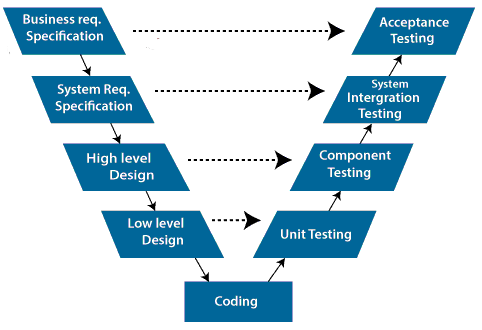
\includegraphics[width=0.7\linewidth]{img/vmodel}
	\caption{Il ciclo di vita dei sistemi: modello a V}
	\label{fig:vmodel}
\end{figure}
\noindent{}A discrezione della fase del ciclo di vita del sistema, si utilizzano differenti tecniche e modelli di validazione: \cite{librobonda}
\begin{itemize}
	\item Specifica: la validazione \`e basata sull'utilizzo di tecniche combinatorie che mirano a determinare le condizioni di fallimento di un sistema in funzione del fallimento dei suoi sottocomponenti, considerati indipendenti;
	\item \emph{Design}: in questa fase si usano modelli analitici \emph{state-based} basati su processi casuali, come ad esempio le Catene di Markov. Si rilassano le assunzioni di indipendenza tipiche dei modelli combinatori;
	\item Implementazione: con il procedere della fase di implementazione, il sistema prende forma e pu\`o essere interessante osservarne direttamente il comportamento per effettuare misure sperimentali. L'attivit\`a di osservazione e misurazione prende il nome di \emph{monitoring};
	\item Fase operativa: il sistema \`e impiegato sul campo e possono essere utilizzate tutte le tecniche disponibili per l'analisi.
\end{itemize}
\subsection{Osservazione dei sistemi}
L'osservazione, o \emph{monitoring}, \`e una tecnica per valutare la \emph{dependability} di un sistema o un suo prototipo osservandone l'esecuzione nell'ambiente finale.\\*
In questa sezione viene esposto il \emph{monitoring} dei sistemi informatici come descritto nei lavori \cite{monitor1}, \cite{monitor2} e \cite{monitor3}.\\*
L'obiettivo \`e quello di monitorare costantemente l'esecuzione del sistema, verificando che il comportamento osservato sia confrome alle aspettative.\\*
Un'attivit\`a di \emph{monitoring} \`e seguita da un'attivit\`a di verifica. Questa pu\`o essere fatta durante l'esecuzione del sistema oppure \emph{offline}, esaminando successivamente i risultati.\\*
Il \emph{monitoring} \`e stato riconosciuto come una valida opzione per valutare gli attributi di \emph{dependability} dei sistemi informatici.\\*
I problemi tecnici da affrontare e risolvere quando si crea un sistema di \emph{monitoring} riguardano:
\begin{itemize}
	\item Individuazione e classificazione degli eventi di interesse, al fine di raccogliere misurazioni utili per valutare correttamente la \emph{dependability} del sistema monitorato;
	\item Trasmissione delle informazioni al luogo dove queste saranno elaborate;
	\item Filtraggio e classificazione degli eventi rispetto alle misure di interesse.
\end{itemize}
Si definisce \emph{target system} il sistema al quale vengono applicate le attivit\`a di \emph{monitoring}. Il componente hardware o software interno al sistema verso il quale si riferisce il \emph{monitoring}, viene detto \emph{target component} o \emph{target application}.\\*
Esistono due differenti configurazioni di un processo di monitoring: \emph{black-box} o \emph{white-box}. Nella configurazione a \emph{black-box} il sistema viene sottoposto a un certo carico di input al fine di osservare l'output prodotto. L'input fornito al sistema prende il nome di \emph{workload}, ed \`e il carico di informazioni che il sistema dovr\`a processare durante il \emph{monitoring}.\\*
\begin{figure}[h]
	\centering
	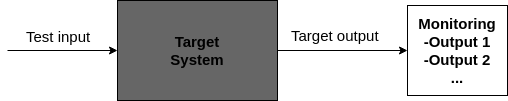
\includegraphics[width=0.7\linewidth]{img/blackbox}
	\caption{Monitoring black-box}
	\label{fig:blackbox}
\end{figure}
\FloatBarrier
Il monitoring \emph{white-box} prevede l'utilizzo agiuntivo di strumenti necessari a osservare anche gli output intermedi che il sistema produce. Questi strumenti sono chiamati sonde, o \emph{probes}.\\*
\begin{figure}[h]
	\centering
	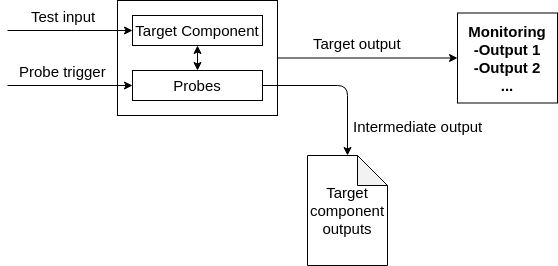
\includegraphics[width=0.7\linewidth]{img/whitebox}
	\caption{Monitoring white-box}
	\label{fig:whitebox}
\end{figure}
\FloatBarrier
I \emph{probes} sono collocati solitamente all'interno del sistema e il loro scopo \`e quello di fornire informazioni pi\`u dettagliate sul comportamento del \emph{target component}.\\*
Se si vogliono monitorare segnali hardware interni al sistema, i \emph{probes} utilizzati saranno effettivamente hardware, mentre si utilizzano \emph{probe} software se si vuole ottenere informazioni sull'esecuzione interna di un programma. Questa tecnica \`e chiamata instrumentazione del codice, e il codice aggiunto prende il nome di \emph{software probe}.\\*
Quando si progetta il \emph{monitoring} di un sistema, si devono rispettare due regole principali:
\begin{itemize}
	\item I \emph{probes} devono essere in grado di raccogliere il giusto numero di informazioni circa il comportamento del sistema;
	\item Il comportamento del \emph{target system} non deve essere alterato in maniera significativa a causa dell'inserimento dei \emph{probes}. Quando questo avviene, si dice che il sistema di monitoraggio \`e \emph{poco intrusivo}.
\end{itemize}
\subsection{Fault Injection}
La \emph{fault injection} \`e un approccio all'analisi della \emph{dependability} che estende le tecniche di \emph{monitoring} esposte in 1.1.2.\\*
\`E definita come la volontaria introduzione di guasti all'interno di un sistema, al fine di osservarne il comportamento in presenza di guasti. \cite{faultinj1} \cite{faultinj2} \cite{faultinj3}\\*

\section{Scopo della Tesi}
Questa Tesi descrive l'attivit\`a di \emph{monitoring} del prototipo di un sistema informatico impiegato nell'ambito del posizionamento ferrotramviario. Per quanto esposto in 1.1.1, il dominio ferrotramviario \`e un contesto \emph{safety-critical}, come tale, lo sviluppo di sistemi informatici da impiegare nell'ambito ferrotramviario \`e regolamentato da specifici standard e requisiti di \emph{dependability}.\\*
Si introducono i sistemi ferrotramviari come derivazione dai classici sistemi ferroviari, si descrive il problema del posizionamento e le tecniche attualmente utilizzate per risolverlo, inquadrando il contesto operativo in cui si colloca il sistema analizzato.
\section{Sistemi Ferroviari e Ferrotramviari}
\`E possibile schematizzare un sistema ferroviario, o ferrotramviario, come un insieme di vetture vincolate a muoversi lungo una traccia fissata.\\*
Questa schematizzazione \`e approssimativamente valida per qualsiasi sistema ferroviario o ferrotramviario, a prescindere dal numero di veicoli transitanti o dall'estensione geografica. Ci\'o che invece differenzia un sistema ferroviario da un sistema ferrotramviario sono:
\begin{itemize}
		\item Le caratteristiche fisiche del veicolo transitante, come lunghezza e massa;
		\item Le caratteristiche geografiche dell'ambiente operativo;
		\item Gli scopi del trasporto.
\end{itemize}
In generale, nel trasporto ferroviario si utilizzano veicoli pesanti atti a trasportare persone o merci su lunghe percorrenze, pertanto \`e comune che l'ambiente operativo di un sistema ferroviario sia prevalentemente extra urbano.\\*
Nel trasporto ferrotramviario, di contro, si utilizzano veicoli leggeri per offrire un'alternativa al cittadino all'utilizzo di mezzi privati durante i suoi spostamenti all'interno di un'area metropolitana. Quest'ultima caratteristica implica che l'ambiente operativo di un sistema ferrotramviario sia radicalmente diverso dall'ambiente operativo di un sistema ferroviario. Le vetture, anche dette \emph{rotabili}, si muovono lungo traccie installate su strade urbane, e di conseguenza il traffico ferrotramviario condivide l'ambiente con il traffico cittadino, come mostrato in figura \ref{fig:tramschema}.\\*
\begin{figure}[h]
		\centering
		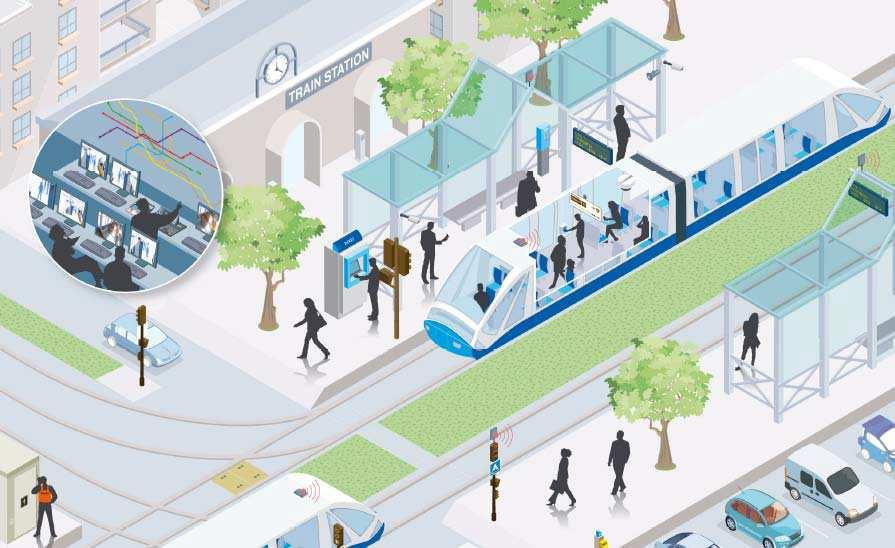
\includegraphics[width=0.7\linewidth]{img/twschema}
		\caption{Schema di un tipico scenario ferrotramviario}
		\label{fig:tramschema}
\end{figure}
\subsection{La safety nei sistemi ferroviari}
La gestione della \emph{safety} nei sistemi ferroviari \`e regolamentata dallo standard \texttt{EN 50126}. \cite{50126}\\*
Questo standard definisce un insieme di documenti che regolamentano la gestione della \emph{safety} nel dominio ferroviario, con particolare enfasi verso le attivit\`a di valutazione RAMS (\emph{Reliability, Availability, Maintainability, Safety}).\\*
Esso prevede che vengano redatti i seguenti documenti.
\paragraph{Safety Plan}\mbox{}\\*Un insieme documentato di attivit\`a programmate, risorse ed eventi necessari a implementare la struttura organizzativa, le responsabilit\`a, le procedure, le attivit\`a, le funzioni e le risorse che insieme assicurano la \emph{safety} del sistema.\\*
In sintesi, il \emph{safety plan} individua \emph{chi} fa \emph{cosa}, e \emph{quando}, al fine di realizzare un sistema \emph{safe}.
\paragraph{Safety Requirements}\mbox{}\\*Definisce i requisiti di \emph{safety} che il sistema deve soddisfare prima di poter essere impiegato sul campo.
\paragraph{Safety Case}\mbox{}\\*La dimostrazione documentata che un prodotto sia conforme ai suoi requisiti di \emph{safety}.
Il \emph{Safety Case} deve essere redatto come una dimostrazione logica della \emph{safety} del sistema.\\*\\*Per quanto riguarda le procedure e i requisiti tecnici per lo sviluppo di applicazioni software utilizzate nel controllo ferroviario, lo standard di riferimento \`e \texttt{EN 50128}. \cite{50128}\\*
Lo standard \texttt{EN 50128} impone che a ciascun software integrato all'interno di un sistema ferroviario debba essere assegnato un livello di \emph{Safety Integrity Level} (SIL). \cite{sil}\\*
Il livello SIL viene assegnato sulla base del tempo medio al fallimento catastrofico, ossia il MTTF relativo a fallimenti catastrofici.\\*
\begin{table}[h]
	\centering
	\begin{tabular}{|l|l|}
		\hline 
		\textbf{Livello SIL} & \textbf{Tempo medio al fallimento catastrofico} \\ 
		\hline 
		\texttt{SIL-1} & $[10^5 - 10^6)$ ore \\ 
		\hline 
		\texttt{SIL-2} & $[10^6 - 10^7)$ ore \\ 
		\hline 
		\texttt{SIL-3} & $[10^7 - 10^8)$ ore \\ 
		\hline 
		\texttt{SIL-4} & $\ge 10^8$ ore \\ 
		\hline 
	\end{tabular} 
\caption{Livelli SIL}
\end{table}
\FloatBarrier
\noindent{}Mentre lo standard \texttt{EN 50126} \`e generico e applicabile a qualunque sistema ferroviario o parti di esso, poich\`e relativo alla \emph{gestione} della \emph{safety} piuttosto che al suo effettivo raggiungimento, lo standard \texttt{EN 50128} \`e inerentemente tecnico e specifico per i software critici.\\*Esso identifica le fasi principali nel ciclo di vita del software e per ciascuna di queste prevede un insieme di tecniche da utilizzare per soddisfare il SIL assegnato al software.
\section{Il problema del posizionamento}
Per posizionamento ferroviario si intende la valutazione della posizione di un treno all'interno di una traccia ferroviaria. Tale posizione viene espressa come progressiva chilometrica rispetto a una posizione nota, come ad esempio l'origine della linea. \cite{trainpositioning}\\*
\subsubsection{Odierne Tecniche di Posizionamento}
Gli odierni sistemi di posizionamento si basano principalmente sull'utilizzo di strumenti installati a terra, chiamati \emph{beacon}, o \emph{balise} in gergo ferroviario, i quali hanno lo scopo di rilevare il passaggio di un treno.\cite{tecnicheodierne}
Esiste uno standard a livello europeo al quale gli odierni sistemi di posizionamento si devono uniformare, l' \emph{European Train Control System} (ETCS).\\*
Nel corso della storia, ogni paese europeo ha sviluppato autonomamente le proprie infrastrutture ferroviarie e relative regole operative. Tuttavia, ad oggi i treni possono attraversare le frontiere, pertanto \`e necessario sviluppare un sistema ferroviario standard che rispetti una comune normativa operazionale europea. Tale sistema prende il nome di \emph{European Rail Traffic Management System} (ERTMS) \cite{ertms}, ed ETCS \`e il sottosistema di ERTMS dedicato al posizionamento delle vetture.\\*
Come standard, ETCS definisce specifici livelli di \emph{compliance} che possiede un sistema di posizionamento rispetto ad ETCS, ed essi vanno dal livello \texttt{ETCS-0} al livello \texttt{ETCS-3}.\\*
L'obiettivo \`e quello di sviluppare progressivamente un sistema di posizionamento completamente autonomo (\texttt{ETCS-3}), partendo da un sistema interamente \emph{non-compliant} con ETCS (\texttt{ETCS-0}).
\\*
Allo stato attuale, quasi tutti i sistemi di posizionamento sono \texttt{ETCS-2}. Nei livelli \texttt{ETCS-1} e \texttt{ETCS-2}, le traccie vengono suddivise in blocchi, e all'entrata di ciascun blocco viene posizionato un \emph{beacon} in grado di rilevare la presenza di un treno.\\*
L'autorizzazione all'ingresso in un blocco viene rilasciata se nessun altro treno sta occupando il blocco al quale si vuole accedere, mentre un sistema di \emph{odometria} installato a bordo, posiziona il treno rispetto all'ultimo \emph{beacon} incontrato.\\*
Nel livello \texttt{ETCS-3}, non sono richiesti segnali provenienti dalla linea: un treno deve essere in grado di posizonarsi autonomamente. \cite{etcs3}\\*
In sintesi, i livelli ETCS possono essere descritti come segue:
\begin{itemize}
	\item \texttt{ETCS-0}: Sistema non conforme a ETCS;
	\item \texttt{ETCS-1}: Utilizzo di apparati di posizionamento installati a terra, autorizzazione a procedere segnalata al macchinista attraverso indicazioni semaforiche;
	\item \texttt{ETCS-2}: Come \texttt{ETCS-1}, ma l'autorizzazione a procedere \`e gestita da un sistema automatico di scambio, denominato sistema di \emph{interlocking};\cite{interlocking}
	\item \texttt{ETCS-3}: Posizionamento autonomo, nessun utilizzo di apparati a terra.
\end{itemize}
\begin{figure}[h]
	\centering
	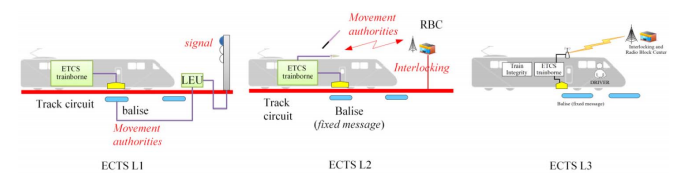
\includegraphics[width=\linewidth]{img/etcs123.png}
	\caption{Livelli \texttt{ETCS}}
	\label{fig:etcs123}
\end{figure}
Il livello \texttt{ETCS-2} prevede che l'autorizzazione a procedere venga gestita dal sistema di \emph{interlocking} e non dal solo operatore umano notificato mediante indicazioni semaforiche.\\*
La funzionalit\`a offerta del sistema di \emph{interlocking} viene pertanto considerata \emph{safety-critical}, in quanto un suo fallimento pu\`o portare a conseguenze anche catastrofiche.\cite{marocchini}\\*
ETCS adotta un approccio incrementale alla realizzazione di sistemi di posizionamento autonomi. Un sistema di posizionamento \texttt{ETCS-3} deve continuare a interagire con il sistema di \emph{interlocking}, quindi deve essere considerato a sua volta un sistema \emph{safety-critical}.\\*
ERTMS/ETCS \`e pensato per sistemi ferroviari, mentre nel dominio ferrotramviario vige la regola della \emph{marcia a vista}. Il rispetto di ETCS non \`e obbligatorio in detto contesto, tuttavia le tecniche di posizionamento ivi utilizzate rispettano spesso le linee guida imposte da ETCS. 
\subsection{Verso ETCS-3}
Gli attuali sistemi di posizionamento richiedono un minimo intervento di computer installati a bordo e una grande quantit\`a di apparati installati a terra. Gli apparati di terra sono costosi e hanno un impatto ambientale non trascurabile, pertanto \`e necessario iniziare a pianificare una migrazione verso sistemi \texttt{ETCS-3}.\cite{market}\\*
Il sistema analizzato in questa Tesi \`e un sottosistema di posizionamento conforme alla filosofia \texttt{ETCS-3}.
\section{Definizione del problema affrontato}
Nell'ottica di migrazione verso sistemi \texttt{ETCS-3}, \`e stato progettato un sistema di posizionamento ferrotramviario autonomo, basato principalmente sull'utilizzo di un \emph{sensore inerziale} installato a bordo treno, le cui misurazioni vengono processate da un sistema software. \cite{svolta}\\*
Attualmente il sistema ha superato le fasi di analisi e definizione dei requisiti, \emph{system design}, e si trova nella fase di implementazione. Si \`e quindi reso disponibile per l'analisi di \emph{dependability} un prototipo del sistema.\\*
Per quanto esposto in 1.1.1, questo pu\`o essere osservato durante l'esecuzione nel suo ambiente operativo.

\chapter{Architettura di Sistema}
In questo capitolo viene descritta l'architettura \emph{hardware} del CPS in esame, in particolare, ne vengono evidenziati i \emph{Constituent System} (CS) e le loro interfacce di comunicazione. Vengono infine descritte le interazioni alle particolari interfacce del sistema.
\section{Descrizione generale}
Lo scopo del sistema \`e quello di implementare un meccanismo di posizionamento basato su SFA.\\*
Il software che esegue tale algoritmo \`e schematizzabile come una \emph{black-box} (figura \ref{fig:sfa}), la quale prende in ingresso un certo insieme di misure, e fornisce in uscita una stima affidabile della posizione del treno lungo la traccia. \cite{datafuse}\\*
\begin{figure}[h]
	\centering
	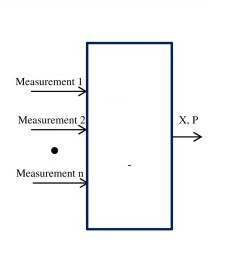
\includegraphics[scale=0.75]{img/sfaschema}
	\caption{Schema SFA}
	\label{fig:sfa}
\end{figure}
\clearpage
Questo algoritmo verr\`a eseguito su di un hardware installato a bordo treno, ed ha lo scopo di monitorare costantemente il moto dello stesso.\\*
Le grandezze fisiche che dovranno essere misurate e fornite a SFA sono:
\begin{itemize}
	\item Vettore accelerazione;
	\item Vettore velocit\`a angolare;
	\item Coordinate geografiche;
	\item Velocit\`a lineare (scalare).
\end{itemize}
In quest'applicazione, SFA utilizza queste informazioni in combinazione con un'apposita digitalizzazione della traccia tramviaria su cui si trova il treno monitorato.\cite{sfaimugps}\cite{sfaimuodo}\cite{sfaimuodogps} \\* Queste informazioni si suppongono note a priori ed accedibili tramite un \emph{database} caricato in memoria centrale. \cite{sqlite3}
\section{Constituent Systems}
Il sistema studiato si compone dei seguenti CS:
\begin{itemize}
	\item \emph{Sensor Set}, ossia un insieme di sensori atto a campionare le misure di interesse per il sistema. Il \emph{Sensor Set} \`e composto dai seguenti moduli:
	\begin{itemize}
		\item \emph{Inertial Measurement Unit} (IMU):\\*
		Unit\`a incaricata di trasmettere al sistema i vettori \texttt{accelerazione} ($\mathbf{a}$) e \texttt{velocit\`a angolare} ($\mathbf{v_{ang}}$). Le misure di IMU sono prese rispetto alla Terra e sono espresse in unit\`a stabilite dallo standard internazionale (SI):
		$$
		\mathbf{a}\;\left[\frac{m}{s^2}\right]\;\;\;\;\mathbf{v_{ang}}\;\left[ \frac{rad}{s} \right]
		$$
		Esso \'e il sensore principale. Date le caratteristiche intrinseche del particolare SFA utilizzato, ossia un \emph{Filtro di Kalman}, il sistema potrebbe funzionare anche senza i rimanenti sensori. Si osserverebbe tuttavia un calo delle performance in termini di errore commesso sulla stima della posizione del treno. \cite{partialmeas} \cite{gpsdarkarea}
		\begin{figure}[h]
			\centering
			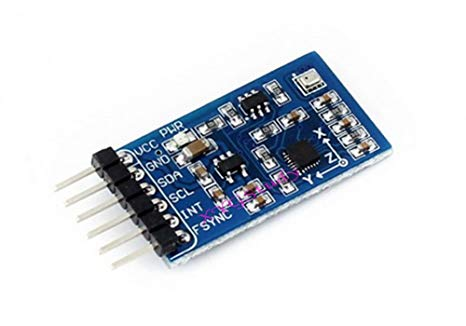
\includegraphics[scale=0.5]{img/imu}
			\caption{\emph{Inertial Measurment Unit}}
			\label{fig:imu}
		\end{figure}
		\item Odometro:\\*
		Unit\`a incaricata di fornire al sistema i campionamenti dei valori di velocit\`a lineare del treno, espressi in $\frac{m}{s}$.
		\item GPS:
		\\*Unit\`a che fornisce al sistema le misure di posizione del treno.\\*
Le misure di GPS sono riportate in formato standard come tripla di coordinate \texttt{(latitudine, longitudine, altitudine)}, rispettivamente espresse in gradi \texttt{N-S}, in gradi \texttt{E-O} e in \texttt{metri} sul livello del mare.
\begin{figure}[h]
	\centering
	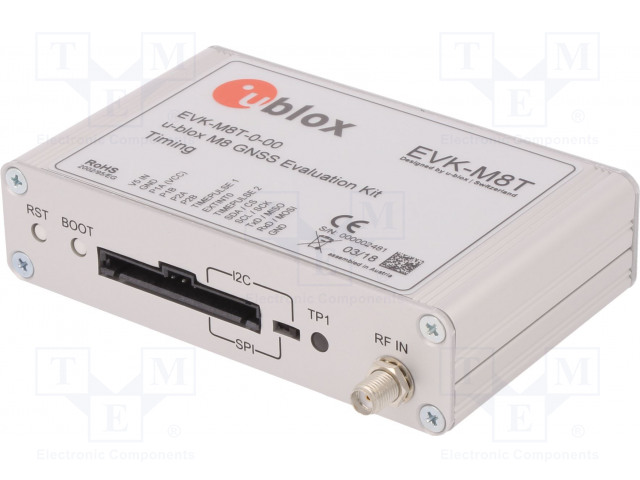
\includegraphics[scale=0.4]{img/gpsublox}
	\caption{Ricevitore \texttt{GPS ublox EVK-M8T}}
	\label{fig:gpsublox}
\end{figure}
\clearpage
	\end{itemize}
	\item Piattaforma di elaborazione dati. Consiste di una scheda \texttt{Nvidia TX-Jetson} su cui viene eseguito SFA.
	\begin{figure}[h]
		\centering
		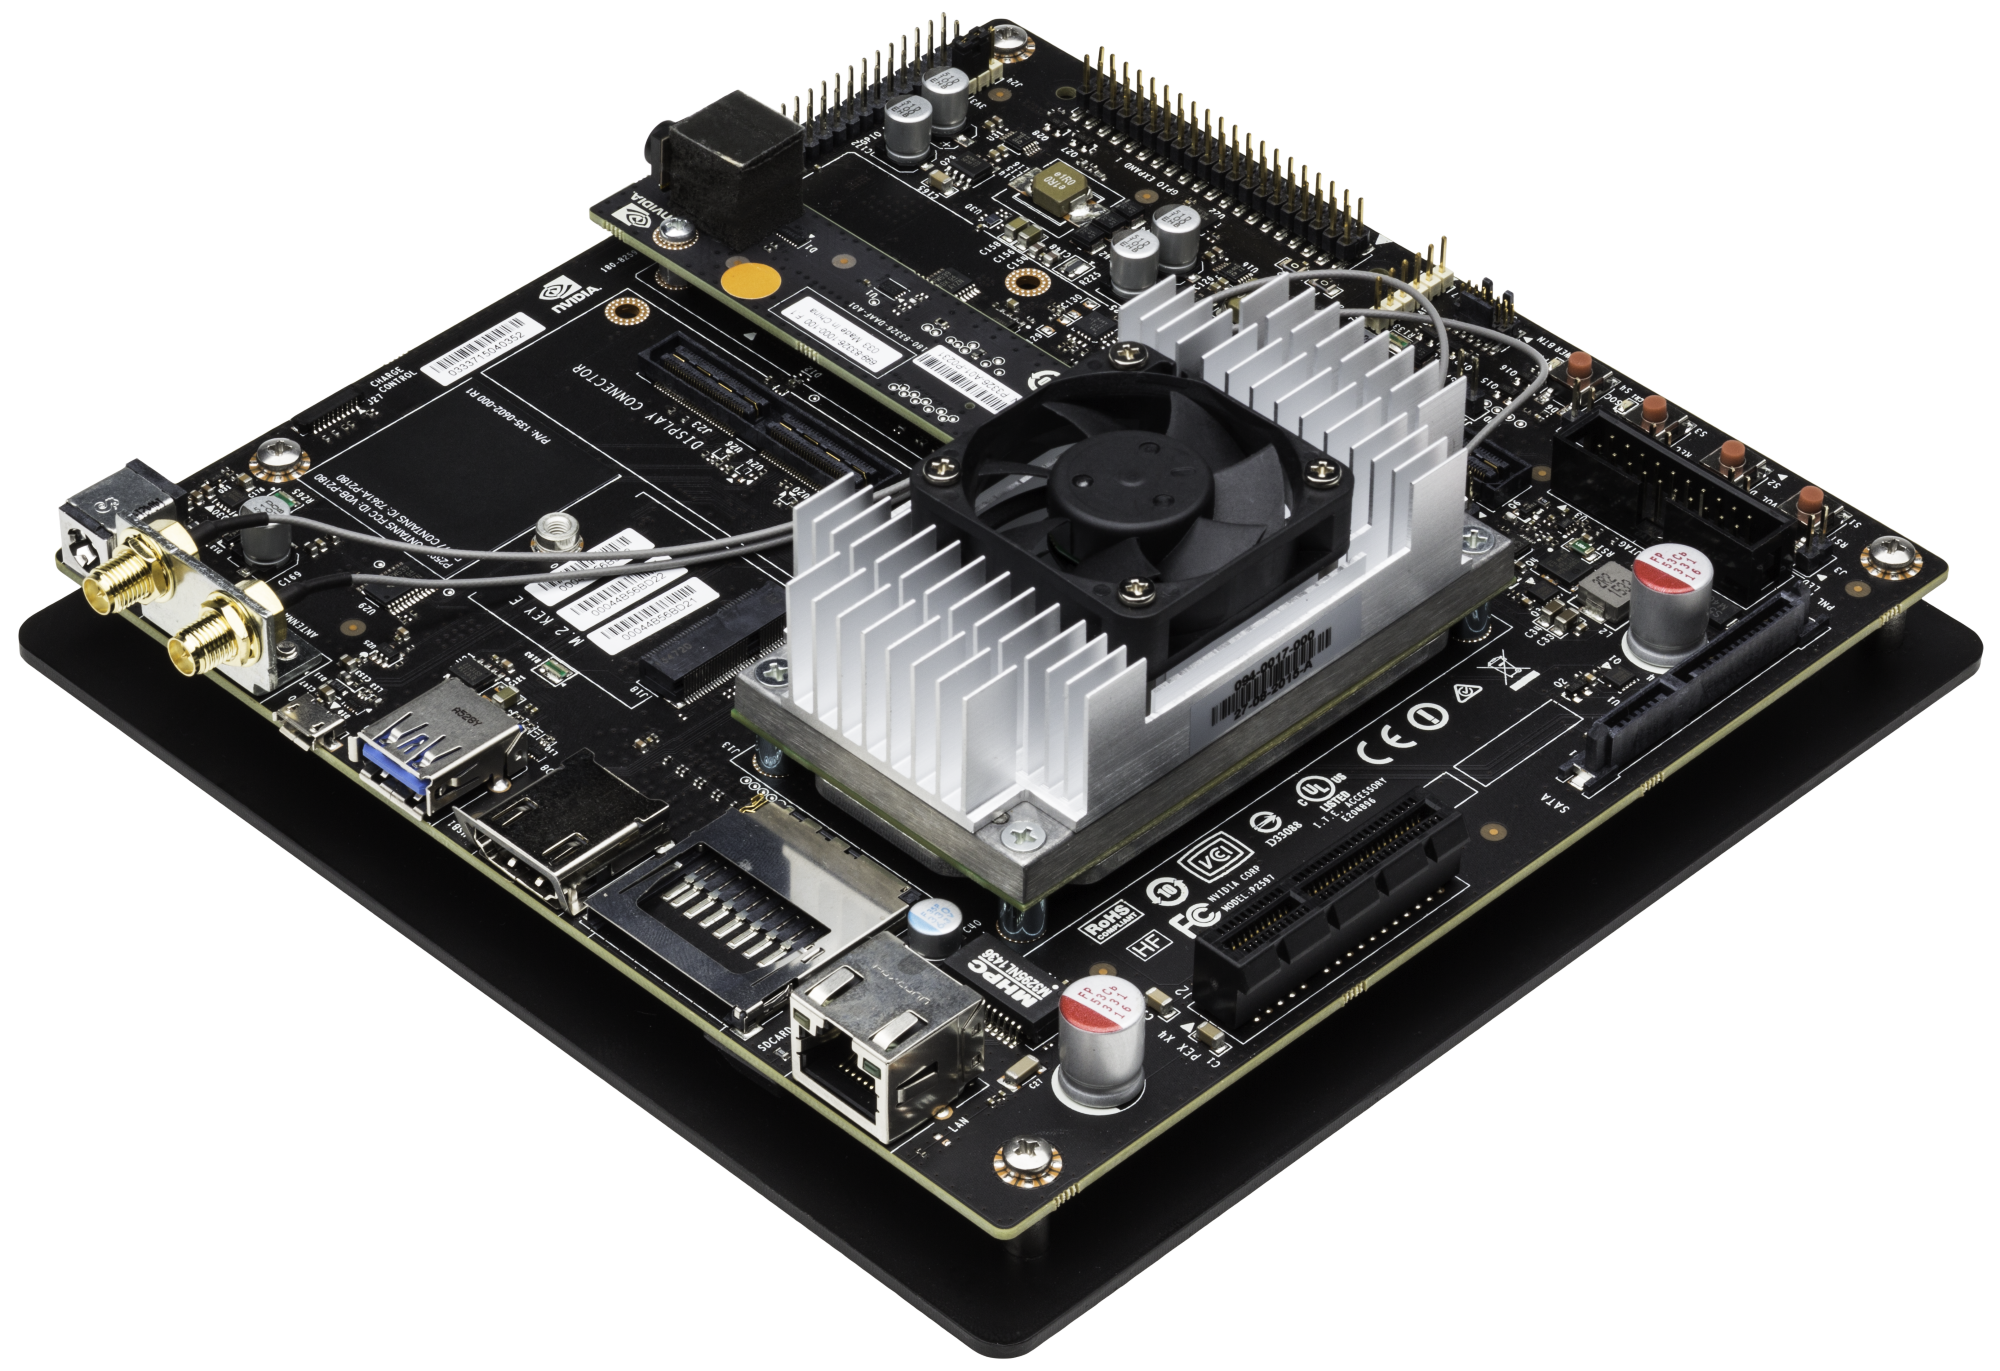
\includegraphics[width=0.7\linewidth]{img/nvidia}
		\caption{\texttt{Nvidia TX-Jetson}}
		\label{fig:nvidia}
	\end{figure}
	\item \emph{On Board Control Unit} (OBCU). Computer di bordo del treno. Esso non svolge alcun ruolo attivo nel sistema di posizionamento, tuttavia la progressiva chilometrica, stimata da SFA, dovr\'a essere trasmessa a OBCU al fine di poter utilizzare questa informazione all'interno del sistema di \emph{interlocking} della traccia.
\end{itemize}
	\section{Specifica delle Interfacce}
	\subsection{Relied Upon Interfaces}
	Le interfacce sono definite come punti di interazione, tra un CS e l'ambiente oppure tra un CS e un altro.\\*
	In questa sezione si evidenziano le principali interfacce del sistema, alle quali si osservano le interazioni fondamentali che avvengono al suo interno.\\*
	Tali interfacce prendono il nome di \emph{Relied Upon Interfaces} (RUI). Le RUI si dividono in:
	\begin{itemize}
		\item \emph{Relied Upon Physical Interfaces} (RUPI), in cui l'interazione avviene tramite osservazione diretta di una grandezza fisica;
		\item \emph{Relied Upon Message Interfaces} (RUMI), dove l'interazione \`e rappresentata da uno scambio di messaggi a livello \emph{cyber}.
	\end{itemize}
	La specifica delle RUI \`e di particolare importanza poich\'e qualunque struttura del sistema, responsabile del comportamento osservato, pu\'o essere ridotta alla specifica delle interfacce del sistema. \cite{interfacespec}.\\*  
	Il CPS interagisce con l'ambiente attraverso le RUPI del \emph{Sensor Set}, ossia gli strumenti di misura che esso integra. Queste interfacce acquisiscono, a diverse frequenze, i dati sul moto del treno che verranno elaborati dal resto del sistema di posizionamento (tabella \ref{tab:rupi}).\\*
	\begin{table}[h]
	\centering
	\begin{tabular}{|c|c|c|}
		\hline 
		\textbf{RUPI} & \textbf{Grandezza Campionata}  & \textbf{Parti interagenti} \\ 
		\hline 
		Accelerometro & Accelerazione & Ambiente - IMU \\ 
		\hline 
		Giroscopio & Velocit\`a angolare & Ambiente - IMU  \\ 
		\hline 
		Radar & Velocit\`a lineare & Ambiente - Odometro \\ 
		\hline 
		Ricevitore GPS & Coordinate geografiche& Ambiente - GPS \\ 
		\hline 
	\end{tabular}
	\caption{Specifica delle RUPI del sistema}
	\label{tab:rupi}
	\end{table}
	Per quanto concerne le RUMI, se ne osservano di due tipi:
	\begin{itemize}
		\item Tre bus dati, che collegano il \emph{Sensor Set} alla scheda \texttt{Nvidia TX-Jetson}. Su ciascuno di essi, \emph{Sensor Set} invia rispettivamente messaggi contenenti i dati campionati da IMU, Odometro e GPS.
		\item Interfaccia LTE. Essa permette di realizzare una \emph{rete wireless ad hoc} fra la scheda e OBCU.\\*
		All'interno di tale rete vengono instradati datagrammi \texttt{IP} contenenti le informazioni sulla progressiva chilometrica stimata da SFA, ed eventualmente messaggi di \emph{acknowledgment} di OBCU verso la scheda.
		\begin{figure}[h]
			\centering
			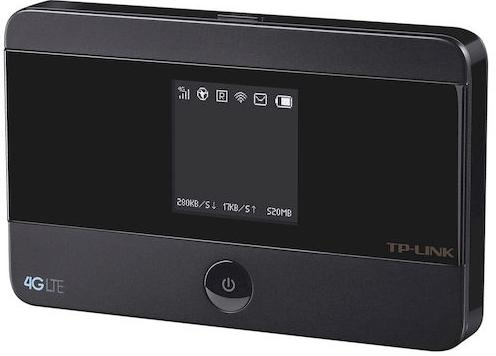
\includegraphics[scale=0.40]{img/lte}
			\caption{Modem \texttt{TP-LINK M7350 LTE-4G}}
			\label{fig:lte}
		\end{figure}
	\end{itemize}
	\begin{figure}[h]
		\centering
		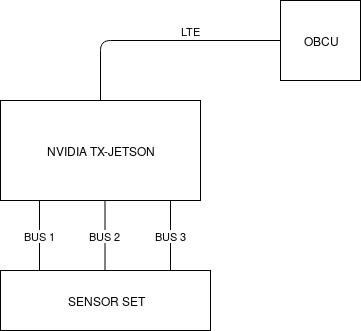
\includegraphics[width=0.7\linewidth]{img/TrainDiagram}
		\caption{RUMI}
		\label{fig:tdiagram}
	\end{figure}
	
	\subsection{Altre Interfacce}
	Oltre alle RUI, descritte in 2.3.1, esistono altre interfacce che hanno lo scopo di rendere il sistema osservabile e manutenibile, e sono le seguenti:	\cite{cecca}
	\begin{itemize}
		\item \emph{Time Synchronization Interfaces} (TSI). Le TSI permettono al CPS di effettuare una sincronizzazione col tempo fisico al fine di stabilire una \emph{global timebase} \cite{clock}.
		\item \emph{Utility Interfaces} (UI). Interfacce dei CS che ne consentono la configurazione, il controllo, e l'osservazione non intrusiva del suo comportamento \cite{monitoring}.
	\end{itemize}
	Come verr\`a approfondito nel successivo capitolo, sia le TSI che le UI sono nella fattispecie interfacce \emph{software}.
	\section{Interazioni}
	In questa sezione vengono descritte le interazioni osservabili alle interfacce del sistema.
	\subsection{Acquisizione dei dati}
	L'acquisizione dei dati si divide in due differenti interazioni: la prima, con l'ambiente, avviene alle RUPI del \emph{Sensor Set}, mentre la seconda avviene alle RUMI di tipo bus dati che collegano il \emph{Sensor Set} alla piattaforma di elaborazione dati.
	I moduli che compongono il \emph{Sensor Set} campionano ad una data frequenza le grandezze fisiche che descrivono il moto del treno. Ciascun campionamento fisico \`e seguito dall'invio dei valori letti alla piattaforma di elaborazione dati. I moduli del \emph{Sensor Set} sono tra di loro indipendenti.\\* 
	\begin{figure}[h]
		\centering
		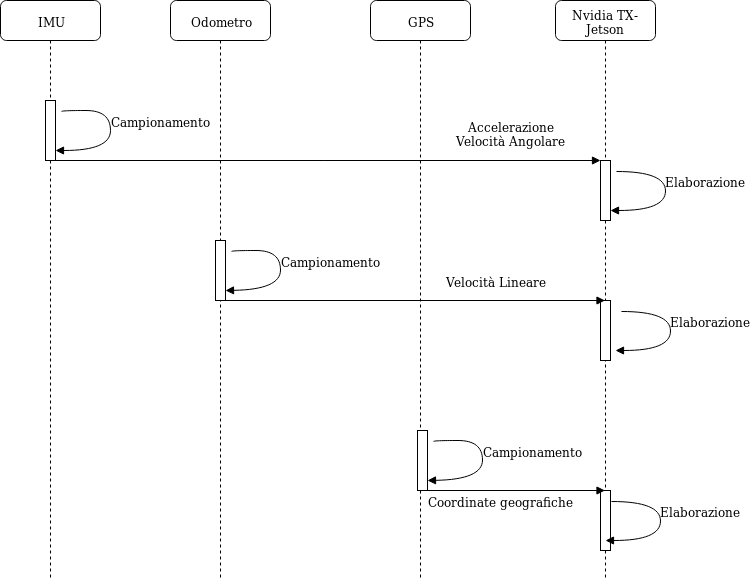
\includegraphics[width=0.7\linewidth]{img/seqdiag}
		\caption{Sequenza di acquisizione dati}
		\label{fig:seqdiag}
	\end{figure}
	In figura \ref{fig:seqdiag} viene riportata una sequenza esempio di campionamento e invio dei dati. I protocolli di comunicazione tra \emph{Sensor Set} e la piattaforma di elaborazione dati sono definiti a livello \emph{software}, e saranno descritti nel prossimo capitolo.
	Questa tipologia di interazione \`e detta \emph{time-triggered}, in quanto \`e determinata unicamente dallo scorrere del tempo. \cite{timetriggered} \cite{evttimetriggered}
	\subsection{Trasmissione della posizione}
	La piattaforma di elaborazione dati esegue SFA durante l'intero moto del treno. Le misure fornite dai sensori vengono elaborate al fine di aggiornare continuamente la stima della posizione del treno.\\*
	Ogniqualvolta un'aggiornamento di SFA viene completato, avviene un'interazione all'interfaccia LTE. Tale interazione consiste nell'invio di un messaggio contenente la posizione del treno, dalla piattaforma di elaborazione dati verso OBCU, e nella trasmissione di un messaggio di \emph{acknowledgment} nel senso opposto.\\*
	La tipologia di scambio dei messaggi esposta \`e detta \emph{event-triggered} \cite{evttimetriggered} in quanto le tempistiche di interazione non sono note a priori, ma dipendono dal tempo impiegato da SFA a compiere un'iterazione per aggiornare la stima prodotta.\\*
	LTE \`e a tutti gli effetti una regolare interfaccia di rete. A livello di trasporto, il messaggio trasmesso \`e contenuto nel \emph{payload} di un datagramma \texttt{UDP}; in accordo al modello di rete \texttt{ISO-OSI}. \cite{libroreti}\\*La specifica del messaggio a livello applicazione sar\`a descritta nel prossimo capitolo.

\chapter{Applicazione di SFA: La Tramvia di Firenze}
In questo capitolo verr\`a analizzata una particolare applicazione di SFA al problema del posizionamento ferrotramviario.\\*
Nell'ambito di un progetto di ricerca finanziato dall'Unione Europea, si \`e voluto studiare l'usabilit\`a di SFA come sistema di posizionamento ferrotramviario alternativo a quello descritto nel Capitolo 1, il quale fa un largo uso di apparati installati a terra, fatto che si vorrebbe minimizzare.\\*
L'idea di base \`e quella di utilizzare UKF per stimare la posizione del treno attraverso misure di accelerazione, velocit\`a angolare, velocit\`a lineare e posizione. La rilevazione di tali grandezze, per quanto esposto nel Capitolo 2, \`e caratterizzata da rumore, UKF combina queste informazioni per stimare la posizione del treno al netto dei rumori di processo e dei rumori di misura.
\section{Architettura di Sistema}
Il sistema progettato ha lo scopo di eseguire SFA su una piattaforma hardware installata bordo treno, la quale riceve i dati \emph{raw} dai sensori e li elabora al fine di stimare la progressiva chilometrica del treno in ciascun istante di tempo.\\*
Tale posizione sar\`a inviata, attraverso un modem \texttt{LTE}:
\begin{itemize}
	\item All'OBCU, per essere utilizzata attivamente all'interno del sistema di \emph{interlocking}
	\item Ad un arbitario host che esegue un software grafico di tracciamento del treno: il \texttt{RailTrackTool} (RTT)
\end{itemize}
\`E possibile descrivere l'architettura di sistema a due differenti livelli: architettura a livello \emph{hardware} e architettura a livello \emph{software}.
\subsection{Architettura Hardware}
Sul treno \`e stata installata una scheda \texttt{Nvidia TX-Jetson} quale piattaforma di elaborazione dei dati. I sensori atti a campionare le misurazioni sono stati collegati alla scheda mediante appositi bus dati.\\*
Il \emph{sensor set} utilizzato in quest'applicazione \`e composto dai seguenti sensori:
 Ad una data frequenza, i sensori inviano dati verso la scheda; quest'ultima, dopo aver eseguito un'iterazione di SFA\footnote{Ossia, un \emph{aggiornamento} di UKF}, invia a OBCU (e/o a RTT) la stima della posizione del treno attraverso apposita modulazione di segnale elettromagnetico, in accordo con il protcollo \texttt{LTE}. Lo schema riportato in figura \ref{fig:tdiagram} mostra un diagramma dell'architettura hardware appena descritta.
\begin{figure}[h]
	\centering
	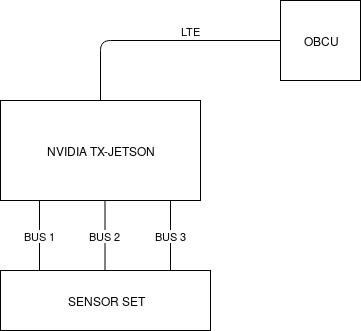
\includegraphics[width=0.7\linewidth]{img/TrainDiagram}
	\caption{Architettura hardware bordo treno}
	\label{fig:tdiagram}
\end{figure}
\subsection{Architettura Software}
Sulla scheda \`e installato il sistema operativo \texttt{Ubuntu 16.04 LTS}, basato su kernel \texttt{Linux}.\\*Qualunque software menzionato in questa Tesi \`e stato sviluppato in linguaggio \texttt{C++}.\\*
Un set di tre moduli software, denominati \texttt{interface-modules}, sono in esecuzione sulla scheda.\\*
Sia MOD\_$i$ l'$i-$esimo modulo software del set e SERIAL\_$i$ l'$i-$esima interfaccia seriale della scheda, per $i = 1,2,3$.\\*
Il funzionamento di \texttt{interface-modules} \`e il seguente:
\begin{itemize}
	\item IMU invia la coppia \texttt{(accelerazione,velocit\`a angolare)} a SERIAL\_1, MOD\_1 legge i valori da SERIAL\_1 e li invia a un secondo modulo software, denominato \texttt{listener}, attraverso l'interfaccia di rete \texttt{loopback}, in quanto \texttt{listener} esegue anch'esso sulla scheda;
	\item Odometro invia il valore di \texttt{velocit\`a lineare} a SERIAL\_2, MOD\_2 legge i valori da SERIAL\_2 e li invia a \texttt{listener};
	\item GPS invia i valori di \texttt{(latitudine, longitudine, altitudine)} a SERIAL\_3, MOD\_3 legge i valori da SERIAL\_3 e li invia a \texttt{listener}.
\end{itemize}
La comunicazione fra \texttt{interface-modules} e \texttt{listener} avviene attraverso un protocollo applicazione stabilito arbitrariamente, sia esso \texttt{INPUT\_PROTOCOL}, mentre a livello di trasporto si utilizza \texttt{UDP}.\\*
I valori ricevuti da \texttt{listener} vengono salvati in apposite \emph{strutture dati} rappresentanti misure della stessa sorgente:
\begin{itemize}
\item I vettori accelerazione e velocit\`a angolare rilevati da IMU vengono convertiti nella struttura dati \texttt{IMU\_POD};
\item La velocit\`a rilevata dal Radar/Odometro viene convertita nella struttura dati \texttt{ODO\_POD};
\item La posizione rilevata dal GPS viene infine convertita nella struttura dati \texttt{GPS\_POD}.
\end{itemize}
Il software che esegue effettivamente SFA \`e compilato come una libreria, \texttt{FusionLib}, utilizzata da \texttt{listener}. \texttt{FusionLib} dispone di interfacce software in entrata e in uscita, ossia \texttt{listener} \`e in grado di inviare le misurazioni a SFA, quali variabili di tipo \texttt{IMU\_POD, ODO\_POD, GPS\_POD} ed altres\'i di ricevere la stima della posizione del treno, essendo questo l'output dell'algoritmo, quale variabile di tipo \texttt{SFA\_OUTPUT\_POD}.\\*
Ogniqualvolta \texttt{listener} riceva un' uscita da SFA, si fa carico della comunicazione tra scheda e OBCU/RTT. Questa comunicazione, fisicamente possibile attraverso l'utilizzo del modem \texttt{LTE}, avviene utilizzando un protocollo di rete arbitrario a livello applicazione, sia esso \texttt{OUTPUT\_PROTOCOL}, mentre al livello di trasporto la scelta \`e nuovamente ricaduta su \texttt{UDP} per ragioni di efficienza.\\*
Uno schema dell'architettura software \`e quello mostrato in figura \ref{fig:tdiagramint}.\\*
\begin{figure}[h]
	\centering
	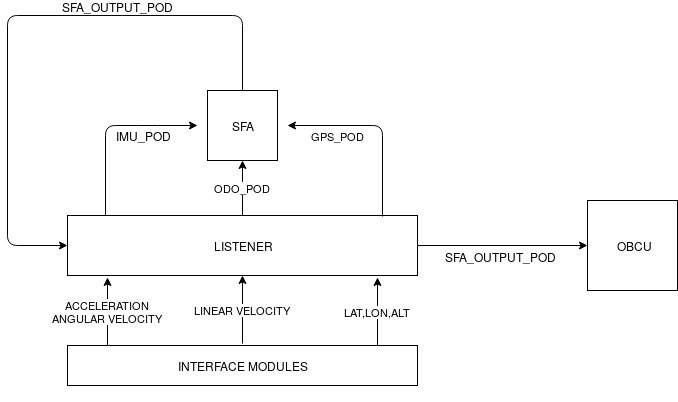
\includegraphics[width=\linewidth]{img/InternalTrainSchema}
	\caption{Architettura software bordo treno}
	\label{fig:tdiagramint}
\end{figure}
\section{Gestione della trasmissione dei dati}
Nella precedente sezione sono stati brevemente introdotti i protocolli di comunicazione implementati per gestire la comunicazione \texttt{UDP}:
\begin{itemize}
	\item In entrata, tra \texttt{interface-modules} e \texttt{listener} (\texttt{INPUT\_PROTOCOL});
	\item In uscita, tra \texttt{listener} e OBCU/RTT (\texttt{OUTPUT\_PROTOCOL}).
\end{itemize}
\subsection{Trasmissione in entrata}
Per trasmettere i dati da \texttt{interface-modules} a \texttt{listener}, e dunque dai sensori al modulo software che implementa SFA, \`e stato realizzato un protocollo di comunicazione denominato \texttt{INPUT\_PROTOCOL}.\\*
Tale protocollo fa affidamento a livello trasporto su \texttt{UDP} per massimizzare la velocit\`a di trasmissione senza dover necessariamente rinunciare all'integrit\`a dei messaggi trasmessi, in quanto la comunicazione avviene tra processi in esecuzione sulla stessa macchina, e la probabilit\`a che un messaggio venga perso o che questo venga ricevuto con errori, \`e assolutamente trascurabile.\\*
Il protocollo definisce il formato del \emph{payload} del pacchetto \texttt{UDP} che contiene le informazioni di IMU, Radar/Odometro, o GPS, ed \`e descritto in tabella \ref{tab:protoin}.\\*
\begin{table}[h]
			\centering
\begin{tabular}{|c|c|c|c|}
	\hline 
	\textbf{Campo} & \textbf{Descrizione} & \textbf{Indici di bit} & \textbf{Tipo} \\ 
	\hline 
	\texttt{SENSOR\_TYPE} & ID Sensore Sorgente & 0-7 & \texttt{uint8\_t} \\ 
	\hline 
	\texttt{Seq.NO} & Numero di sequenza & 8-23 & \texttt{uint16\_t} \\ 
	\hline 
	\texttt{N\_INT} & Numero di interi trasmessi & 24-31 & \texttt{uint8\_t} \\ 
	\hline 
	\texttt{N\_DOUBLE} & Numero di double trasmessi & 31-38 & \texttt{uint8\_t} \\ 
	\hline 
\end{tabular} 
\caption{Protocollo di comunicazione in entrata}
\label{tab:protoin}
\end{table}
A discrezione del valore del campo \texttt{SENSOR\_TYPE} si distingue il tipo di informazione trasportata dal pacchetto, come descritto in tabella \ref{tab:sensors}.\\*
\begin{table}[h]
		\centering
	\begin{tabular}{|c|c|}
		\hline 
		\textbf{Valore di SENSOR\_TYPE} & \textbf{Sorgente del pacchetto} \\ 
		\hline 
		$1$ & IMU \\ 
		\hline 
		$2$ & ODOMETRO \\ 
		\hline 
		$3$ & GPS \\ 
		\hline 
		$8$ & GROUND TRUTH \\ 
		\hline 
		$9$ & STROBE \\ 
		\hline 
		$10$ & STOP \\ 
		\hline 
	\end{tabular} 
	\caption{Significato del campo SENSOR\_TYPE}
	\label{tab:sensors}
\end{table}
I pacchetti \texttt{GROUND TRUTH} sono pacchetti di inizializzazione dell'algoritmo: alla ricezione del pacchetto \texttt{GROUND TRUTH} l'algoritmo si avvia leggendo i valori trasmessi in coda al pacchetto, in accordo al valore dei campi \texttt{N\_INT} e \texttt{N\_DOUBLE}. Tali valori forniscono informazioni come progressiva chilometrica e velocit\`a iniziali del treno.\\*
I pacchetti \texttt{STROBE} sono inviati ogni secondo e forniscono un solo valore \texttt{double}, ossia un \texttt{timestamp} che l'algoritmo utilizza per sincronizzarsi.\\*
Il pacchetto \texttt{STOP} non contiene alcuna informazione utile: indica soltanto all'algoritmo di terminare l'esecuzione.\\*
Alla ricezione di un pacchetto, \texttt{listener} legge il valore del campo\\*\texttt{SENSOR\_TYPE}, e costruisce, in accordo alla relazione sorgente-struttura dati, la variabile da inviare a SFA.\\*
Il corretto ordinamento dei pacchetti trasmessi a SFA \`e garantito attraverso l'esplicito utilizzo di un buffer, codificato all'interno di \texttt{listener}, in cui i pacchetti vengono temporaneamente salvati prima di essere inviati a SFA, ed eventualmente ordinati sulla base del valore del campo \texttt{Seq.NO}.\\*
Si osservi che se l'integrit\`a non \`e minacciata dall'utilizzo di \texttt{UDP} quale protocollo di trasporto fra processi all'interno della stessa macchina fisica, altrettanto non si pu\`o dire dell'ordinamento dei messaggi. Questi potrebbero subire dei ritardi casuali in base allo stato del sistema operativo, in particolare lo \emph{scheduling} dei processi pu\`o avere influenze determinanti sullo scorretto ordinamento dei messaggi trasmessi. Utilizzando \texttt{TCP} si ovvierebbe a questa problematica, ma l'overhead insito nel protocollo stesso causerebbe un notevole degrado delle performance di SFA.
\subsection{Trasmissione in uscita}
La trasmissione dei dati in uscita da SFA avviene, in accordo al protocollo \texttt{OUTPUT\_PROTOCOL} tra \texttt{listener} e OBCU, o comunque, tra \texttt{listener} e qualunque host arbitrario che intenda ricevere le informazioni in uscita, come ad esempio un \texttt{PC} sul quale viene eseguito RTT.\\*
Come specificato, la comunicazione \`e posta in essere, a livello fisico, attraverso il protocollo \texttt{LTE}, ossia un un protocollo \emph{wireless}; mentre a livello trasporto si \`e scelto di continuare a usare \texttt{UDP} in luogo di \texttt{TCP}, col fine di massimizzare le \emph{performance} del sistema.\\*Il rischio di ricevere alcune informazioni in maniera errata, o non riceverle del tutto, \`e nettamente pi\`u elevato rispetto allo scenario precedente, nel caso in cui lo spazio fisico attraverso cui si propaga il segnale \texttt{LTE} \`e tale per cui quest'ultimo venga disturbato da sorgenti esterne.\\* Gli effetti deleteri di questa condizione sono particolarmente osservabili in alcuni tratti della linea ferrotramviaria, dove possono essere presenti numerose abitazioni e mezzi di trasporto in strada che si interpongono fisicamente tra la scheda \texttt{NVidia TX-Jetson} su cui esegue SFA e l'arbitrario host su cui viene eseguito RTT.\\*Occorre tuttavia osservare che il tracciamento del treno tramite RTT non \`e in alcun modo legato alla \emph{safety} del sistema, in quanto le funzionalit\`a \emph{safety-critical} riguardano la comunicazione tra la scheda e OBCU, ossia tra la scheda e il sistema di \emph{interlocking}.\\*
Questa problematica \`e risolta attraverso l'esplicito utilizzo di un meccanismo di \texttt{acknowledgment} simile a quello utilizzato da \texttt{TCP}: ciascun pacchetto in uscita da SFA viene indicizzato con un \emph{sequence number} e, in ricezione, viene inviato ogni secondo un \emph{ack} replicante l'ultimo numero di sequenza correttamente ricevuto. Solo quando il mittente riceve l'ack $i$ dal destinatario invier\`a il messaggio contenente l'uscita indicizzata con \emph{sequence number} $i+1$.\\*
Anche in questo caso, il protocollo definisce il formato del \emph{payload} del pacchetto \texttt{UDP} inviato da \texttt{listener}, ed \`e riportato in tabella \ref{tab:protoout}.\\*
\begin{table}[h]
	\centering
	\begin{tabular}{|c|c|c|c|}
		\hline 
		\textbf{Campo} & \textbf{Descrizione} & \textbf{Indici di bit} & \textbf{Tipo} \\ 
		\hline
		\texttt{Seq.NO} & Numero di sequenza & 0-15 & \texttt{uint16\_t} \\ 
		\hline 
		\texttt{ECEF\_X} & Coordinata X del treno & 16-79 & \texttt{double} \\ 
		\hline 
		\texttt{ECEF\_Y} & Coordinata Y del treno & 80-143 & \texttt{double} \\ 
		\hline 
		\texttt{ECEF\_Z} & Coordinata Z del treno & 144-207 & \texttt{double} \\ 
		\hline 
		\texttt{FU\_ARC\_LEN} & Progressiva chilometrica & 208-271 & \texttt{double} \\ 
		\hline 
	\end{tabular} 
\caption{Protocollo di comunicazione in uscita}
\label{tab:protoout}
\end{table}
In ricezione dovr\`a essere inviato il pacchetto \emph{ack} al mittente, ed il suo formato \`e descritto in tabella \ref{tab:ack}.
\begin{table}[h]
	\centering
	\begin{tabular}{|c|c|c|c|}
	\hline 
	\textbf{Campo} & \textbf{Descrizione} & \textbf{Indici di bit} & \textbf{Tipo} \\ 
	\hline
	\texttt{ACK} & Ultimo \texttt{Seq.NO} & 0-15 & \texttt{uint16\_t} \\ 
	\hline
\end{tabular}
\caption{Formato del pacchetto di \emph{ack}}
\label{tab:ack}
\end{table}
Si osserva che SFA produce la stima della posizione del treno sia in termini di progressiva chilometrica che di coordinate \texttt{ECEF}.\\*
\texttt{ECEF} \`e acronimo di \emph{Earth Centered Earth Fixed} ed \`e uno standard che misura le coordinate geografiche di un oggetto come la terna $ P = (x,y,z)$. Ciascuna coordinata viene espressa considerando la \emph{proiezione su piano} della Terra, e prendendo come origine $O$ l'intersezione fra l'equatore e il meridiano di \emph{Greenwich}.\\*
Le coordinate \texttt{ECEF} misurano tre lunghezze, pertanto, in accordo a SI, esse sono espresse in \texttt{metri}.\\*
Nella prossima sezione, viene descritto uno scenario di esempio del comportamento del sistema a \emph{runtime}.
\section{Scenario di Esempio}
Si suppongano le condizioni iniziali riportate in tabella \ref{tab:condinit}.\\*
\begin{table}[h]
	\centering
	\begin{tabular}{|c|c|c|c|c|}
		\hline 
		\textbf{Velocit\`a} & \textbf{ECEF} & \textbf{Progressiva} & \textbf{IMU Sample Rate} & \textbf{ODO Sample Rate} \\ 
		\hline 
		$0ms^{-1}$ & $(0, 0, 0)$ m & 0 km & 100 Hz & 20 Hz \\ 
		\hline 
	\end{tabular} 
	\caption{Condizioni iniziali}
	\label{tab:condinit}
\end{table}
\begin{enumerate}
	\item $t = 0$:\\*
	\begin{itemize}
	\item \texttt{interface-modules} invia a \texttt{listener} il seguente pacchetto \texttt{GROUND TRUTH}:\\*\\*
	\begin{tabular}{|c|c|c|c|}
		\hline 
		\textbf{SENSOR\_TYPE} & \textbf{Seq. NO} & \textbf{N\_INT} & \textbf{N\_DOUBLE} \\ 
		\hline 
		\texttt{0x08} & \texttt{0x00} & 0 & 5 \\ 
		\hline 
	\end{tabular}\\*\\*
	E vi accoda i seguenti tre valori \texttt{double: 0.0, 0.0, 0.0} ossia le coordinate \texttt{ECEF} iniziali, il seguente valore \texttt{double: 0.0}, ossia la velocit\`a lineare iniziale, e infine il valore \texttt{double: 0.0} che rappresenta la progressiva chilometrica iniziale.
	\item \texttt{listener} riceve il pacchetto e inizializza SFA con:
	\begin{itemize}
		\item \texttt{ECEF} iniziali: $(0, 0, 0)$
		\item Velocit\`a lineare iniziale: $0.0$
		\item Progressiva chilometrica iniziale: $0.0$
	\end{itemize}
	\end{itemize}
	\item $t=t_0$:\\*
	\begin{itemize}
	\item IMU campiona il seguente vettore accelerazione:
	$$
	\mathbf{a} = (0.0001, -0.0001, -9.8100)
	$$
	Assieme al seguente vettore velocit\`a angolare:
	$$
	\mathbf{v_{ang}} = (0.0003, -0.0001, 0.0002)
	$$
	E lo invia, tramite \texttt{SERIAL\_1}, a \texttt{MOD\_1} di \texttt{interface-modules}.
	\item \texttt{MOD\_1} invia a \texttt{listener} il seguente pacchetto \texttt{IMU}:\\*\\*
		\begin{tabular}{|c|c|c|c|}
		\hline 
		\textbf{SENSOR\_TYPE} & \textbf{Seq. NO} & \textbf{N\_INT} & \textbf{N\_DOUBLE} \\ 
		\hline 
		\texttt{0x01} & \texttt{0x01} & 0 & 6 \\ 
		\hline 
	\end{tabular}\\*\\*
	Accodandovi nell'ordine il vettore accelerazione, e il vettore velocit\`a angolare.
	\item \texttt{listener} riceve il pacchetto, crea e invia a SFA la seguente variabile \texttt{IMU\_POD}:
	\begin{itemize}
		\item \texttt{Seq.NO = 1}
		\item \texttt{Epoch = $t_0$}
		\item \texttt{ACC\_X = 0.0001}
		\item \texttt{ACC\_Y = -0.0001}
		\item \texttt{ACC\_Z = -9.8100}
		\item \texttt{GYRO\_X = 0.0003}
		\item \texttt{GYRO\_Y = -0.0001}
		\item \texttt{GYRO\_Z = 0.0002}
	\end{itemize}
\item SFA elabora il pacchetto e inizia una computazione parallela per fornire a \texttt{listener} una variabile \texttt{SFA\_OUTPUT\_POD} della forma:
	\begin{itemize}
		\item \texttt{Seq.NO = 0}
		\item \texttt{ECEF\_X = }$E_X$
		\item \texttt{ECEF\_Y = }$E_Y$
		\item \texttt{ECEF\_Z = }$E_Z$
		\item \texttt{FU\_ARC\_LEN = }$P_{KM}$
	\end{itemize}
	\end{itemize}
	\item $t_0 < t < t_0 + \frac{1}{ODO\_SAMPLE\_RATE} = t_0 + \frac{1}{20}$\\*
	Fintantoch\'e l'odometro non campiona il suo primo valore di velocit\`a, si ripetono le operazioni viste al passo precedente per ogni campionamento di \texttt{IMU}.
	\item $t = t_0 + \frac{1}{20}$\\*
		\begin{itemize}
		\item Odometro campiona il seguente valore di velocit\`a:
		$$
		\mathbf{a} = (1.0010)
		$$
		E lo invia, tramite \texttt{SERIAL\_2}, a \texttt{MOD\_2} di \texttt{interface-modules}.
		\item \texttt{MOD\_2} invia a \texttt{listener} il seguente pacchetto \texttt{ODOMETRO}:\\*\\*
		\begin{tabular}{|c|c|c|c|}
			\hline 
			\textbf{SENSOR\_TYPE} & \textbf{Seq. NO} & \textbf{N\_INT} & \textbf{N\_DOUBLE} \\ 
			\hline 
			\texttt{0x02} & \texttt{Seq\_{NO}} & 0 & 2 \\ 
			\hline 
		\end{tabular}\\*\\*
		Accodandovi nell'ordine il valore di velocit`a rilevato, e il valore dello scarto quadratico medio della sorgente, noto a priori, in quanto caratteristica tecnica intrinseca dello strumento di misura, il radar; sia esso \texttt{SIGMA\_{RADAR}}.\\*
		\item \texttt{listener} riceve il pacchetto, crea e invia a SFA la seguente variabile \texttt{ODO\_POD}:
		\begin{itemize}
			\item \texttt{Seq.NO = Seq\_{NO}}
			\item \texttt{Epoch = $t_0 + \frac{1}{20}$}
			\item \texttt{vel = 1.0010}
			\item \texttt{sigma = SIGMA\_{RADAR}}
		\end{itemize}
		\item SFA elabora il pacchetto e utilizza la rilevazione di velocit\`a in maniera utile a correggere il \emph{drift} di IMU, al fine di produrre una stima della posizione pi\`u accurata.
		\end{itemize}
	\item $t = n\;t_0\;\;\;\;\;\;\;n \in \mathbb{N}^+$\\*
	Ogni secondo, il modulo \texttt{STROBE} di \texttt{interface-modules}, invia a \texttt{listener} un pacchetto della forma:
	\\*\\*
	\begin{tabular}{|c|c|c|c|}
		\hline 
		\textbf{SENSOR\_TYPE} & \textbf{Seq. NO} & \textbf{N\_INT} & \textbf{N\_DOUBLE} \\ 
		\hline 
		\texttt{0x09} & \texttt{Seq\_{NO}} & 0 & 1 \\ 
		\hline 
	\end{tabular}\\*\\*
Accondandovi un \emph{timestamp} che \texttt{listener} inoltra a SFA per scopi di sincronizzazione.
\end{enumerate}
Quanto elencato viene ripetuto per ciascun campionamento successivo di IMU e odometro.\\*
Nonappena un' uscita di SFA si rende disponibile a \texttt{listener} questo si comporta come segue:
\begin{itemize}
	\item \texttt{listener} riceve la variabile \texttt{SFA\_OUTPUT\_POD}, da SFA;
	\item \texttt{listener} costruisce il seguente pacchetto da inviare a OBCU, o a RTT:
		\begin{itemize}
		\item \texttt{Seq.NO = 0x00}
		\item \texttt{ECEF\_X = } \texttt{SFA\_OUTPUT\_POD.}$E_X$
		\item \texttt{ECEF\_Y = } \texttt{SFA\_OUTPUT\_POD.}$E_Y$
		\item \texttt{ECEF\_Z = } \texttt{SFA\_OUTPUT\_POD.}$E_Z$
		\item \texttt{FU\_ARC\_LEN = } \texttt{SFA\_OUTPUT\_POD.}$P_{KM}$
	\end{itemize}
	\item OBCU, o RTT, riceve il pacchetto e invia a \texttt{listener} l'\emph{ack} \texttt{0x00}.
\end{itemize}
\section{Possibili sviluppi}
Il sistema, cos\'i come \`e stato descritto, rappresenta essenzialmente un \emph{core} minimale di un sistema di posizionamento basato su SFA, limitato rispetto alle potenzialit\`a dell'algoritmo e comunque non esente da vulnerabilit\`a legate alla \emph{security}. In questa sezione verranno discusse le principali problematiche della soluzione descritta, in che modo queste possono essere risolte, e quali tecniche possono essere usate per migliorare l'usabilit\`a del sistema.
\subsection{Problematiche legate alla security}
Per \emph{security} si intende un insieme di tecniche che hanno come scopo la protezione dei dati, siano essi stoccati in un sistema informatico, oppure transitanti attraverso un sistema di telecomunicazione.\\*
Tale protezione viene assicurata contro specifiche \emph{minacce}, le quali sfruttano opportune \emph{vulnerabilit\`a}.\\*
La \emph{security} viene garantita attraverso l'uso di appropriate \emph{tecniche preventive}, oppure \emph{contromisure} applicabili in caso di violazioni alle principali \emph{misure} della \emph{security}:
\begin{itemize}
	\item Integrit\`a
	\item Confidenzialit\`a
	\item Autenticazione
\end{itemize}
In un sistema \emph{safety-critical} come quello descritto, una violazione di \emph{security} potrebbe portare a una violazione di \emph{safety}, pertanto \`e fondamentale ridurre al minimo le vulnerabilit\`a del sistema.
Nella fattispecie descritta in questa Tesi, tuttavia, la confidenzialit\`a non \`e una misura fondamentale, mentre lo sono l'integrit\`a e l'autenticazione.
\subsubsection{Minacce all'integrit\`a}
\`E stato gi\`a discusso che l'utilizzo del protocollo \texttt{UDP} a livello di trasporto, non garantisce affatto che i messaggi ricevuti da OBCU siano corretti e ordinati.\\*
Per ovviare al problema dell'ordinamento \`e stato implementato il gi\`a descritto meccanismo di \texttt{acknowledgment}, tuttavia esso fa l'implicita assunzione che se si \`e in grado di leggere correttamente il numero di sequenza del pacchetto ricevuto, questo non sia stato alterato.\\*
Si consideri il seguente scenario:
\begin{itemize}
	\item \texttt{listener} invia a OBCU il seguente pacchetto:
	\begin{itemize}
		\item \texttt{Seq.NO = 0x17}
		\item \texttt{ECEF\_X = } \texttt{SFA\_OUTPUT\_POD.}$E_X$
		\item \texttt{ECEF\_Y = } \texttt{SFA\_OUTPUT\_POD.}$E_Y$
		\item \texttt{ECEF\_Z = } \texttt{SFA\_OUTPUT\_POD.}$E_Z$
		\item \texttt{FU\_ARC\_LEN = } \texttt{SFA\_OUTPUT\_POD.}$P_{KM}$
	\end{itemize}
	\item OBCU riceve il seguente pacchetto:
\begin{itemize}
	\item \texttt{Seq.NO = 0x25}
	\item \texttt{ECEF\_X = } \texttt{SFA\_OUTPUT\_POD.}$E_X$
	\item \texttt{ECEF\_Y = } \texttt{SFA\_OUTPUT\_POD.}$E_Y$
	\item \texttt{ECEF\_Z = } \texttt{SFA\_OUTPUT\_POD.}$E_Z$
	\item \texttt{FU\_ARC\_LEN = } \texttt{SFA\_OUTPUT\_POD.}$P_{KM}$
\end{itemize}
\end{itemize}
Per come \`e stato descritto il protocollo, OBCU accetta passivamente che il numero di sequenza ricevuto sia \texttt{0x25}, anche se prima di questo era stato letto il valore \texttt{0x16}, ed invier\`a a \texttt{listener} l'\emph{ack} \texttt{0x25}.\\*
In questo caso, OBCU dovrebbe essere progettato in maniera tale da controllare sempre di ricevere un numero di sequenza pari all'ultimo ricevuto $+1$. Dal momento che, viste le caratteristiche intrinseche del protocollo, \`e impossibile che \texttt{listener} abbia inviato il pacchetto con numero di sequenza \texttt{0x25} se l'ultimo \emph{ack} ricevuto non era \texttt{0x24}, \`e probabile che, attraversando il canale, il pacchetto abbia subito alterazioni casuali in tutti i suoi bit, e quindi anche l'informazione di posizione potrebbe essere alterata.\\*
Per ovviare definitivamente alla problematica dell'integrit\`a, \`e opportuno integrare nel protocollo l'uso di una \emph{funzione hash}. Il protocollo verrebbe modificato come segue:
\begin{itemize}
	\item \texttt{listener} prepara il pacchetto contenente le informazioni di\\* \texttt{SFA\_OUTPUT\_POD};
	\item \texttt{listener} calcola \texttt{H(SFA\_OUTPUT\_POD) = y};
	\item \texttt{listener} invia la coppia \texttt{(SFA\_OUTPUT\_POD,y)}
\end{itemize}
In ricezione, OBCU ricalcola \texttt{H(SFA\_OUTPUT\_POD) = y'}, e accetta il messaggio solo se \texttt{y' = y}. Infatti, grazie alla propriet\`a delle funzioni \emph{hash}, una minima variazione del messaggio $m$ causa una grande variazione del \emph{digest} $H(m)$, quindi \`e altamente improbabile che un'alterazione casuale dei bit trasmessi, sia essa \texttt{(SFA\_OUTPUT\_POD\_WRONG, Y\_WRONG)}, mantenga la propriet\`a \texttt{H(SFA\_OUTPUT\_POD\_WRONG) = Y\_WRONG}.
\subsubsection{Minacce all'autenticazione}
Si consideri il caso in cui un malintenzionato sia in grado di inviare messaggi a OBCU e abbia interesse nel non segnalare al sistema di \emph{interlocking} l'avvicinamento del treno alla JA.\\*
L'attaccante si comporta come segue:
\begin{itemize}
	\item Intercetta il messaggio \texttt{(SFA\_OUTPUT\_POD,H(SFA\_OUTPUT\_POD))}
	\item Modifica la posizione del treno ponendola lontano da una JA, forgiando un nuovo messaggio, sia esso \texttt{SFA\_OUTPUT\_POD\_DANGEROUS}
	\item Calcola \texttt{H(SFA\_OUTPUT\_POD\_DANGEROUS) = Y\_DANGEROUS}
	\item Invia a OBCU la coppia \texttt{(SFA\_OUTPUT\_POD\_DANGEROUS, Y\_DANGEROUS)}
\end{itemize}
Per ovviare a questa problematica si potrebbero usare le seguenti tecniche:
\begin{enumerate}
	\item Cifratura del \emph{digest} della funzione \emph{hash} con una chiave simmetrica condivisa tra \texttt{listener} e OBCU;
	\item Cifratura del \emph{digest} della funzione \emph{hash} con la chiave privata di \texttt{listener} (Firma Digitale \texttt{DSA});
	\item Uso di una funzione \emph{hash} che prende in ingresso sia il messaggio che una chiave simmetrica condivisa tra \texttt{listener} e OBCU (\texttt{HMAC});
	\item Accodare un segreto condiviso tra \texttt{listener} e OBCU al messaggio prima di calcolarne il \emph{digest}.
\end{enumerate}
In ciascuno di questi scenari, fatta assunzione di propriet\`a di \emph{strong collision resistance} della funzione \emph{hash} utilizzata, si garantisce che il messaggio pu\`o essere stato inviato solo da \texttt{listener}, in quanto un attaccante non avrebbe modo di modificare il messaggio e calcolare un \emph{digest} valido. La soluzione meno dispendiosa in termini di complessit\`a computazionale e pi\`u adatta a un simile scenario \`e la soluzione 4, in quanto non \`e necessario garantire anche la \emph{non-ripudiabilit\`a} ma solo l'autenticazione e l'integrit\`a.
\subsection{Miglioramenti al protocollo in uscita}
Il sistema realizzato esegue una versione di SFA basata su un UKF.\\*
Ad ogni campionamento di IMU, Odometro, o GPS, viene eseguita la fase di \emph{aggiornamento} del filtro che comprende la valutazione di quantit\`a interessanti dal punto di vista di valutazione delle \emph{performance} dell'algoritmo. In particolare, si potrebbe analizzare il comportamento di SFA al variare di parametri come:
\begin{itemize}
	\item La frequenza di aggiornamento;
	\item Il tipo di misure con cui viene effettivamente aggiornato il filtro.
\end{itemize}
Nel classico scenario di utilizzo, che comprende la comunicazione con OBCU, l'unica informazione effettivamente utile \`e la progressiva chilometrica.\\* In uno scenario di \emph{acceptance test}, naturalmente preliminare al rilascio del sistema, potrebbe essere utile fornire a RTT, oltre alle informazioni sulla posizione, anche i valori in entrata all'algoritmo che hanno prodotto il risultato di posizione.\\*
Inoltre, se fosse trasmessa anche la matrice di covarianza della stima a posteriori, verrebbero fornite indicazioni importanti sul comportamento qualitativo dell'algoritmo.\\*
Queste modifiche comporterebbero una minima variazione di\\*\texttt{OUTPUT\_PROTOCOL} in quanto occorrerebbe semplicemente prevedere dei campi aggiuntivi al formato del pacchetto, che si aggiungerebbero ai campi relativi alle coordinate ECEF e alla progressiva chilometrica.


\chapter{Ambiente di Analisi}

\chapter{Esperimenti e Risultati}
Questo capitolo rappresenta la parte sperimentale del lavoro di Tesi.\\*
Si illustrano gli esperimenti condotti sul sistema nell'ambiente descritto nel capitolo 4, e si discutono i risultati ottenuti.
\section{Traccia di analisi}
La traccia ferrotramviaria scelta per l'analisi \`e un sottoinsieme della linea \texttt{T1} della Tramvia di Firenze.\\*
\`E stato scelto un sottoinsieme della linea, in luogo della linea intera, principalmente per ragioni di complessit\`a computazionale.
\section{Misure di interesse}
Prima di poter procedere all'analisi del sistema, occorre definire le \emph{misure di interesse} che si intende valutare attraverso gli esperimenti condotti.
\chapter{Conclusioni}
In questa Tesi, si \`e discusso un processo di analisi sperimentale condotto verso un sottosistema di posizionamento ferrotramviario.\\*
L'analisi condotta rientra nella categoria \emph{fault injection}, che prevede l'osservazione diretta del sistema, o di un suo prototipo, nel suo reale ambiente di esecuzione. Il fine di un'attivit\`a di \emph{fault injection} \`e quello di raccogliere accurate misure sperimentali circa la \emph{dependability} del sistema analizzato, quando vengono inseriti volontariamente dei guasti al suo interno. Si \`e discusso il concetto di \emph{dependability}, definendola come la capacit\`a che ha un sistema di fornire un servizio in modo corretto. In particolare, sono stati individuati:
\begin{itemize}
	\item Le \emph{measures}, ovvero i parametri di valutazione della \emph{dependability};
	\item I \emph{threats}, ossia gli eventi che minano la \emph{dependability} di un sistema;
	\item I \emph{means}, insieme di tecniche e metodologie atte a raggiungere la \emph{dependability} di un sistema informatico.
\end{itemize}
La \emph{dependability} \`e un aspetto fondamentale per tutti i sistemi informatici, ma il suo raggiungimento diventa obbligatorio per sistemi operanti in contesti \emph{safety critical}, come ad esempio il settore ferroviario.\\*
Sono stati discussi gli standard \texttt{EN 50126} e \texttt{EN50128} che regolamentano la gestione e il raggiungimento della \emph{safety} nei sistemi ferroviari, e le normative operazionali imposte dallo standard europeo \texttt{ERTMS/ETCS}, completando il quadro del contesto normativo e operativo in cui si colloca il sistema studiato.\\*
Il sistema \`e stato poi classificato, da un punto di vista architetturale, come un \emph{Cyber Physical System of Systems}, quindi se ne sono descritti gli elementi architetturali, come le interfacce e i sistemi costituenti. La descrizione del sistema si \`e quindi conclusa con la specifica dei sistemi software che lo compongono.\\*
Definito il sistema nominale, la discussione si \`e concentrata sulla descrizione dell'ambiente di analisi costruito al fine di garantire le propriet\`a, note dalla letteratura, che un sistema di \emph{monitoring} e \emph{fault injection} deve possedere.\\*
Sono stati quindi descritti gli esperimenti condotti individuando:
\begin{itemize}
	\item Un \emph{fault model} rappresentativo per il sistema;
	\item Le misure di interesse che si intende valutare;
	\item Un \emph{workload} il pi\`u possibile conforme agli input reali che il sistema dovr\`a processare;
	\item Un \emph{faultload} basato sui requisiti di sistema e sulle tecnologie usate.
\end{itemize}
I risultati che ha fornito la campagna di \emph{fault injection} sembrano promettenti nell'ottica di poter impiegare il sistema sul campo, sebbene questo sia ancora in fase di sviluppo e si \`e reso disponibile per l'analisi solamente un suo prototipo.\\*
\begin{thebibliography}{9}

\bibitem{trainpositioning}
J. Otegui, \textit{A Survey of Train Positioning Solutions, IEEE Sensors Journal, Vol. 17, No. 20 (2017)}

\bibitem{tecnicheodierne}
T. Albrecht et al, \textit{A precise and reliable train positioning system and its use for automation of train
operation, Proc. IEEE Int. Conf. Intell. Rail Transp. (2013)}

\bibitem{ertms}
European Commission, \textit{
	Delivering an effective and interoperable European Rail Traffic Management System
	(ERTMS) - the way ahead (2017)}

\bibitem{svolta}
J. Marais, J. Beugin, M. Berbineau, \textit{A Survey of GNSS-Based Research and
	Developments for the European Railway Signaling, IEEE transactions on intelligent transportation system (2017)}

\bibitem{etcs3}
A. Neri, F. Rispoli, P. Salvatori, \textit{An analytical assessment of
a GNSS-based train integrity solution in typical ERTMS level 3
scenarios, in Proc. Eur. Navigat. Conf. (ENC), Bordeaux, France, (2015)}

\bibitem{interlocking}
 P. Josserand, F.H Willard, \textit{Rights of Trains (5th ed.),Simmons-Boardman Publishing Corporation, New York (1957)}
 
\bibitem{marocchini}
N.A. Zafar et al, \textit{Towards the safety properties of moving blockrailway interlocking system, International Journal of Innovative Computing Information and Control (2012)}

\bibitem{MISRA}
MISRA, \textit{MISRA-C:2004, Guidelines for the use of the C language in critical systems (2004)}

\bibitem{sil}
International Electrotechnical Commission, \textit{61508-1: Functional safety of electrical/electronic/programmable electronic safety-related systems, edition 2.0 (2010)}


\bibitem{50128}
CENELEC European Committee for Electrotechnical Standardization. \textit{EN 50128:2011 - Railway Applications - Communications, signalling and processing systems - Software for railway control and protections systems (2011)}

\bibitem{market}
R. S. Hosse, H. Manz, K. Burmeister, E. Schnieder, \textit{Market
analysis for satellite train localisation for train control systems,
Proc. 5th Conf. Transp. Solutions Res. Deployment Transp. (2014)}
\bibitem{cps}
D. Basile et al, \textit{A Refinement Approach to Analyse Critical Cyber-Physical Systems,
Software Engineering and Formal Methods  (2017)}

\bibitem{cecca}
A. Ceccarelli et al, \emph{Basic Concepts on Systems of Systems, Cyber-Physical Systems of Systems, Springer (2017)}


\bibitem{sfarailway}
A. Mirabadi et al, \textit{Application of sensor fusion to railway systems, IEEE (1996)}

\bibitem{datafuse}
F. Bohringer, A. Geistler, \textit{Adaptation of the kinematic train
	model using the interacting multiple model estimator, Advances in
	Transport, vol. 74, no. 7. Southampton (2004)}

\bibitem{sfaimugps}
B. Cai, X. Wang, \textit{Train positioning via integration and
fusion of GPS and inertial sensors, WIT Transactions on the Built Environment, Southampton (2000)}

\bibitem{sfaimuodo}
M. Malvezzi et al, \textit{A localization algorithm for railway vehicles based on sensor fusion between tachometers and inertial measurement units, Proc. Inst. Mech.}

\bibitem{sfaimuodogps}
C. Reimer et al, \textit{INS/GNSS/odometer
data fusion in railway applications, Proc. DGON Intertial Sensors
Syst. (ISS), vol. 2. Karlsruhe, Germany (2016)} 

\bibitem{sqlite3}
L. Junyan et al, \textit{Application Research of Embedded Database SQLite, IEEE (2009)}

\bibitem{partialmeas}
X. Liu, A. Goldsmith, \textit{
Kalman  Filtering with Partial Observation Losses, Department of Electrical Engineering, Stanford University, Stanford, USA}

\bibitem{gpsdarkarea}
R. Mazl, L. Preucil, \textit{Sensor Data Fusion for Inertial Navigation of
Trains in GPS Dark Areas (Mathematics in Science and Engineering),
San Diego, CA, USA (2003)}

\bibitem{nvidia}
S. Mittal, \textit{A Survey on optimized implementation of deep learning models on the NVIDIA Jetson platform, Journal of Systems Architecture
Volume 97 (2019)}
	

\bibitem{interfacespec}
H. Kopetz, \textit{Real-Time Systems: Design Principles for Distributed Embedded Applications 2nd edn, Springer, New York (2011)}

\bibitem{clock}
H. Kopetz, W. Ochsenreiter, \textit{Clock synchronization in distributed real-time systems, IEEE (1987)}

\bibitem{monitoring}
K. Wolter et al,
\textit{Resilience Assessment and Evaluation of Computing Systems, Springer (2012)}

\bibitem{timetriggered}
M.J. Pont, \emph{Patterns for Time-Triggered Embedded Systems, Addison-Wesley (2001)}

\bibitem{evttimetriggered}
H. Kopetz, \emph{Event-Triggered versus Time-Triggered Real-Time Systems, Springer (1991)}

\bibitem{libroreti}
ISO/IEC 7498-1:1994, \textit{
Information technology, Open Systems Interconnection - Basic Reference Model: The Basic Model (1994)}

\bibitem{librokalman}
D.E. Katlin, \textit{Estimation, Control, and the Discrete Kalman Filter, Applied Mathematical Science, Springer (1987)}

\bibitem{measnoise}
S. Dilhaire, D. Maillet, \textit{Dealing  with the measurement noise of a sensor (2015)}

\bibitem{mocking}
M. Karlesky et al, \textit{Mocking the Embedded World,
Test-Driven Development, Continuous Integration, and Design Patterns
Embedded Systems Conference, Silicon Valley (San Jose, California)
(2007)}

\end{thebibliography}



%--------------------------------------------------------------
\end{document}
%--------------------------------------------------------------